\documentclass[hyperref,english,bachelorofscience,bibnum,twoside]{cgvpub}
%weitere Optionen zum Erg�nzen (in eckigen Klammern):
% 
% bibnum	numerische Literaturschl�ssel
% final 	f�r Abgabe	
% lof			Abbildungsverzeichis
% lot			Tabellenverzeichnis
% noproblem	keine Aufgabenstellung
% notoc			kein Inhaltsverzeichnis
% twoside		zweiseitig
\author{Daniel Bekele}
\title{Interactive Registration of 3D Scans in VR}
\birthday{15th January 1995}
\placeofbirth{Jena}
\matno{309845}
\betreuer{Prof. Dr. Stefan Gumhold}
\bibfiles{new_literature_DB}
\problem{
\section{Motivation and Goals:}
When 3D scanning real objects several scans from different views need to be acquired and combined. For high quality reconstruction of a surface model, the relative 3D scanner poses of the different views need to be determined accurately before combining the points from the individual 3D scans. This process is also called registration. The registration problem can be split into coarse and fine registration. In coarse registration a registration with low accuracy is determined which is further refined by a fine registration, for which fully automatic methods work efficiently. The goal of the thesis is to study the coarse registration problem in an interactive setting where a user adjusts the relative poses in a VR environment and to compare its efficiency with a WIMP based interface, e.g. the one implemented in MeshLab [].
\section{Tasks:}
\begin{itemize}
\item Literature research on registration approach with a focus on interactive and semi-automatic approaches
\item Collection of a representative set of 3D scan collections
\item Design of a VR environment for the interactive registration realizing the concept of a workbench and a natural alignment of the 3D scan collection that needs to be registered in a way the selection of individual scans is efficient.
\item Implementation of VR-based picking and positioning strategy of individual point clouds based on the interaction capabilities of a VIVE VR set.
\item Development and implementation of a strategy to guide the user through the process of registering all scans of a dataset
\item Integration of an automatic fine registration algorithm like SparseICP [].
\item Evaluation of the developed methods in a qualitative user study based on a ground truth dataset provided by the Chair of Computer Graphics and Visualization.
\end{itemize}
\section{Optional Tasks:}
\begin{itemize}
\item Integration of a surface reconstruction algorithm in a background process to preview the reconstructed surface based on the current intermediate registration result
\item Design and implement specific interactions and visualizations that help in a faster or more accurate user based registration
\item Improvement of the realism of the VR environment by integrating detailed and textured 3D models.
\end{itemize}
}
\copyrighterklaerung{Hier soll jeder Autor die von ihm eingeholten
Zustimmungen der Copyright-Besitzer angeben bzw. die in Web Press
Rooms angegebenen generellen Konditionen seiner Text- und
Bild"ubernahmen zitieren.}
\acknowledgments{I would like to thank Prof. Dr. Gumhold for his guidance and patience during this thesis. Especially for his help with the framework and the VR interface that made this thesis possible.
I would also like to thank my roomates for the help as test persons and their help with questions and constant reminders that my time is short. Further more I would like to thank the chair of computer graphics for providing the ground truth data.}
\abstracten{This bachelor thesis provides a short introduction into the field of 3D scan registration with a focus on interactive registration techniques. The main goal was to investigate if a VR envorinment for coarse registration alignment is an efficient method and to develop such an application. In addition to this, an user interaction strategy was developed and is examined in detail. This application was then tested in a quality user study and evaluated. The results showed an accurate coarse alignment with an average of 70-120mm translation error and 6\textdegree - 10\textdegree rotation error. The test persons rated the provided interaction interface good with minor improvments to be done. This thesis is interesting for persons interested in VR technology and interaction concepts as well as for the field of 3D scan registration with semi automatic methods.}

\begin{document}

\chapter{Introduction}
During the past 30 Years a rapid development in the field of  virtual and augmented reality took place. The technology itself was not new and invented even earlier, but less affordable for users at home. Due to the lack of computational power of home PCs early systems for VR were not available for most people. With the drop of hardware prices and a rising gaming industry things changed soon and the technology is now available for early adopters. Within a few more years it is to be expected that most people will gain access to VR systems

As the shipment of VR systems exceeded the threshold of 4 Million sold units in 2018 (see ~\ref{fig:sales})\cite{statisticaVR18} VR clearly has the possibility to become a mainstream medium for entertainment. But its purpose is not restricted to this field, as its capability to produce a replica of normally hard accessible objects and even inner organs of humans enables it to provide a perspective view on things that are not visible otherwise. Even objects that are non-existent in the real virtual at the given moment can be reproduced and examined with this technology. This property is especially useful for real time CAD applications. In near future there is the chance that designing 3D objects will take place in Virtual Reality rather than on 2D screens that use a projection of the 3D virtual world on a plane.

In order to successfully apply such construction techniques, some scientific problems need to be solved first. One of these is the 3D registration problem, commonly known in the field of computer graphics, as well as in robotics, medicine and CAD Applications.
This thesis goal is to conduct research in previous attempts for solutions of this problems which include user interaction, as well as to develop an interactive 3D registration program. Finally a user study should provide more useful insights on the interactive registration process in virtual reality.

\chapter{3D scan registration}

As an introduction to the topic this first chapter will briefly define the registration problem as well as it will introduce related work in the field of interactive registration. The second part will provide the mathematical background of registration algorithms.

The registration problem is defined as finding the matching transformation for one set of data to match to a target set of data\cite{Ji2017}. These sets of data are mostly point clouds, but are not limited to them, as the problem can be extended to meshes and surfaces or even pictures\cite{Salvi2007}.
This task can be splitted into the coarse and fine registration, the first one is a rough guess, the second one the actual registration that brings both data as close as possible.
In order to work properly, or to achieve faster and better results, most registration algorithms require a coarse registration that is done before the fine registration algorithm starts. 
\begin{quote}
"Depending on the method used, a quite accurate initial
guess is required because some methods have convergence
problems due to the presence of local minima."\cite{Salvi2007}
\end{quote}

To ensure the registration does not stuck in a local minima different methods have been developed, however the following chapter will focus on related work which includes interactive methods to solve the coarse alignment problem.

\section{Related Work}

As introduction to the field of interactive registration and in order to gain information of the general idea, this section will focus on examining related work. Fully automated algorithms for the registration problem mostly need 2 different algorithms for coarse and fine alignment. As an example shown in a paper by Ji \cite{Ji2017} an improved method of the ICP for fine alignment and a genetic algorithm for coarse alignment is used. The current research in this shows a tendency for fully automated algorithms, interactive methods are rare cases.

An important work to mention is a semi automatic approach of Chao, who used feature based methods for automated registration and to reduce rotation errors the user is involved by choosing the correct rotation.\cite{Chao}
In the first step of their method, an automated registration is executed. After that happened, the result is shown to the user and he can chose to keep the alignment if it is correct, otherwise he can correct the initial rotation. The possible rotation options are limited due to a precalculation step that determines the possible rotations via heuristics. The rotations are then restrained to the axis of the scenery.\cite{Chao}

The experiments conducted along with the tests of this method showed positive results:
Whenever the fully automated initial registration failed, errors were eliminated by user interaction and all scans were aligned. The needed time differed whether much user interaction was needed or not and how many features that disturbed the automated algorithm the scans contained.

Another paper proposed a more user interaction dependent method in 1994.
The 3D image registration for validation of several medical scans was proposed along with an interactive coregstration algorithm by an article of Uwe Pietrzy et a\cite{Pietrzyk1994}. The main goal was to align scans of brains with a reference scan in order to detect anomalies, which may indicate a disease of the patient. The corregstration is mainly driven by user interaction and achieved accurate results that put up to the fully automated techniques of that time. Additionally the algorithm was far less restricted than the automated techniques, which needed different assurances to work. Figure 2.1 shows the workflow of the application developed by them.
\begin{figure}[htbp]
	\centering
		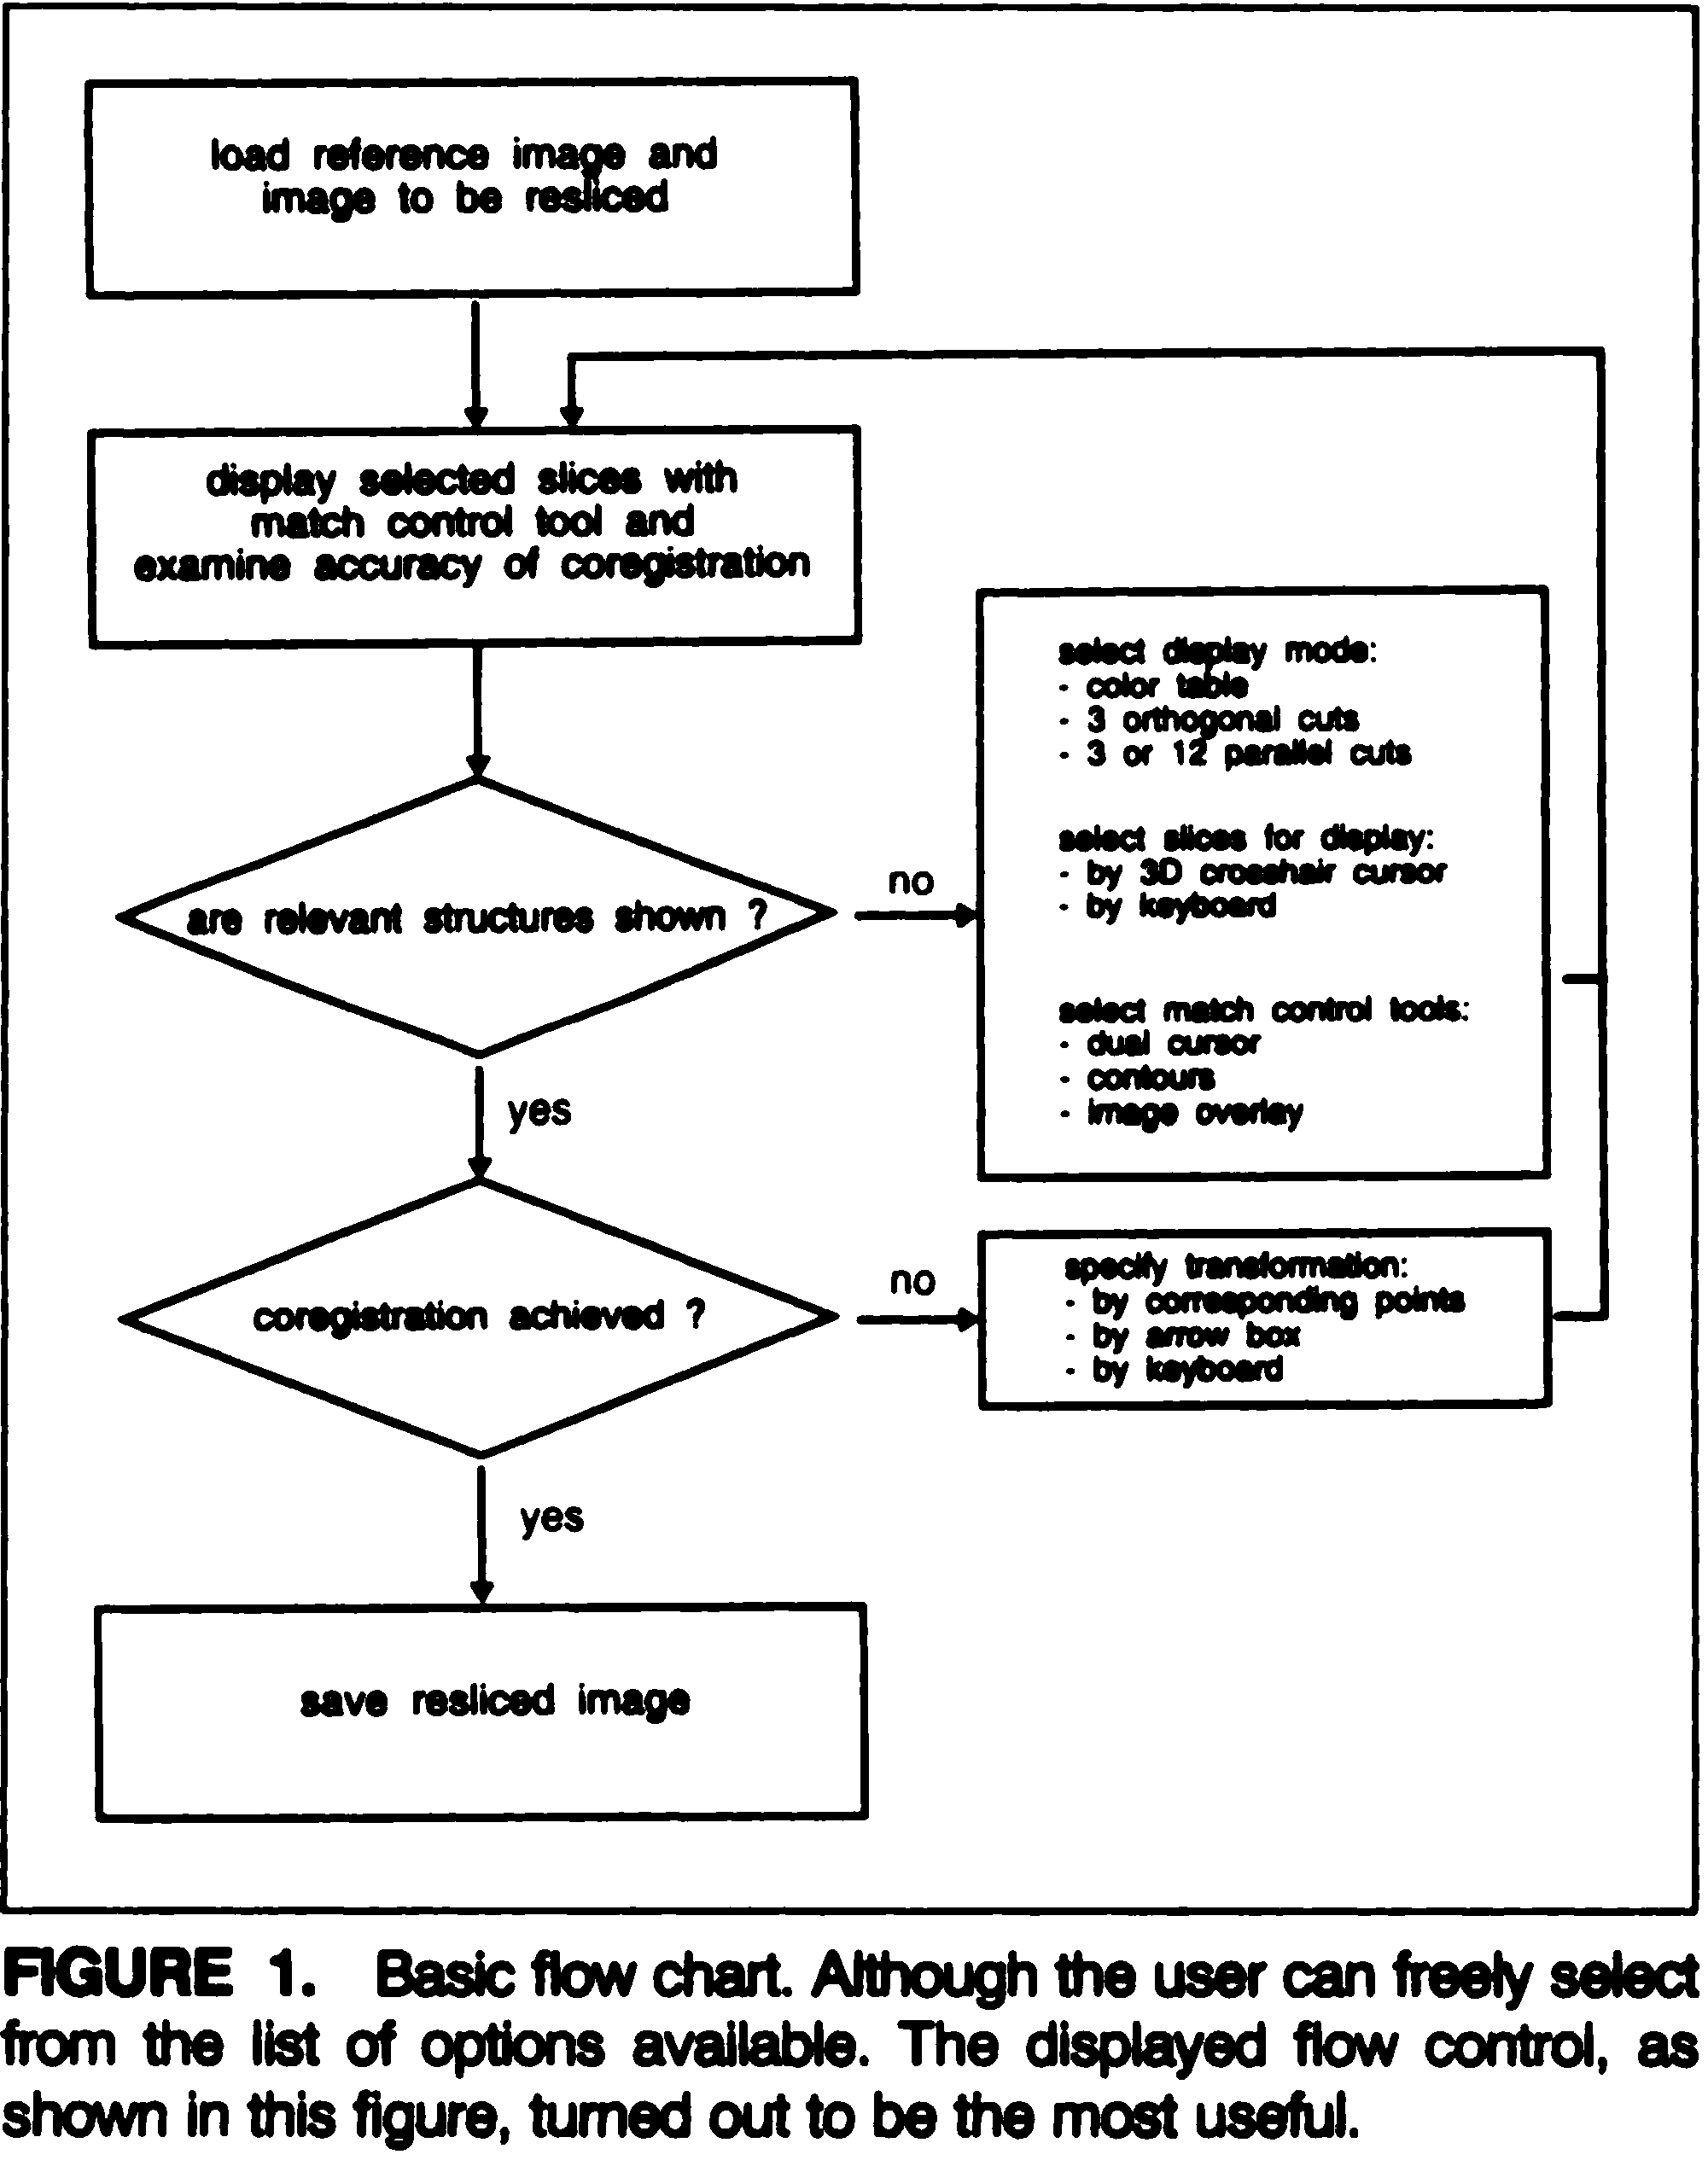
\includegraphics[width= \linewidth]{flow_chart_uwe_p.png}
	\caption{The workflow of the application\cite{Pietrzyk1994}}
	\label{fig:workflow}
\end{figure}

\section{Introduction to registration algorithms} \label{sec:Itra}

In order to solve the registration problem, different strategies have been developed. The first step, the coarse alignment, can be done by user interaction or other specialized algorithms. The second step of fine registration needs an algorithm, because interactive methods cannot achieve as accurate results as the registration done by computers. This chapter should provide an insight to the fine registration problem, especially its solution through a commonly used algorithm. First the prerequisites are examined, then the Iterative closest point algorithm (ICP) is explained as an example for the solution of the registration problem.

To achieve this goal of fine registration the task can be splitted into several steps:
\begin{enumerate}
\item  Find corresponding points between the roughly aligned sets of data
\item  Find a formula to retrieve the transformation needed to align dataset A to dataset B using the correspondences found in 1.
\item Calculate the actual transformation.
\item Apply the actual transformation
\end{enumerate}

\subsection{Correspondences}

To find corresponding points between 2 sets of points a fast and efficient method is needed, hence this study is focused on user interaction which is disturbed if an algorithm would need long times and the surrounding application does not respond.
The k-nearest neighbour search (knn-search) is commonly used for such problems, as its includes the distances between the nearest points and should deliver good results, given the scans are near together and approximately have the correct rotation. The circumstances of the application fulfil this requirements, since it needs the user to coarse align the scans before the automated fine alignment.
The knn-search calculates, as its name implies, the distance to the nearest points. To estimate the nearest neighbours, distances between the individual points need to be calculated and then sorted to find the closest points.

Given this situation a simple knn-search with the brute Force method fails. The method would calculate all distances between all points, the resulting complexity of  \textit{O(mnd)} \cite{Garcia2008}, with m as number of all points from the first point cloud and n with the number of all points from the second point cloud. d is the number of nearest points that are obtained and stored. This does not meet the requirement of the application to work in real time with point clouds with a higher number of points.
To enhance the efficiency of this method many different acceleration data structures have been introduced. The one used in the actual implementation of the application for this thesis is the so called KD-tree, which will be explained in the next sections.

\subsection{KD-Trees}

\begin{quote}
"k-d trees are a generalization of binary search trees."\cite{Nuchter2007}
\end{quote}
In theory this means that all points are represented by a binary tree structure. The root node contains the whole point cloud. The variable k defines the dimensions which is 3 in our example, hence we are working in 3D space when aligning scans. This variable can be higher if e.g. the colours of scans are as additional information available.
Building such a tree has an average runtime in the complexity of \mbox{\textit{O(log n)}, to optimize it \textit{O(n log n)}\cite{bentley1975}}.

Their main advantage is their runtime for knn-querys: 
\begin{quote}
"for nearest neighbor queries [empirically observed average running time of \textit{O(log n)}.]" \cite{bentley1975}
\end{quote}
Using KD-trees for a knn-query results in a much better performance since building such a tree and using it costs less than using brute force method. Additionally through parallelization the actual runtime can further be reduced. The code excerpt below shows a snippet which uses a KD-tree for a knn-query executing parallel. This implementation is used during the execution of the fine alignment of the version of the ICP which was tested during development. The code is taken from the stanford university.

\begin{figure}[htbp]
\begin{lstlisting}[frame=trbl]
           /// Find closest point
           #pragma omp parallel for
            for(int i=0; i<X.cols(); ++i) {
               Q.col(i) = Y.col(kdtree.closest(X.col(i).data()));
           }
\end{lstlisting}
\end{figure}

Newer researches have shown that cached KD-trees algorithms using GPU programming have better results\cite{Garcia2008}, this will not be the case in our application since the GPU is fully occupied by providing a rendered stereoscopic view and the ICP was removed due to several problems. See ~\nameref{ch:Problems} for details.
The resulting correspondences can now be used to calculate a rigid-body transformation that aligns two point clouds. To achieve this many applications rely on a commonly known algorithm called Iterative closest point (ICP).

\subsection{The iterative closest point algorithm}

\begin{quote}
"ICP starts with two meshes and an initial guess for their relative rigid-body transform, and iteratively refines the transform by repeatedly generating pairs of corresponding points on the meshes and minimizing an error metric."\cite{Rusinkiewicza}
\end{quote}
In the test during the development the Transformation is a translation and a rotation matrix that when applied to the point cloud aligns it to the target point cloud.

The initial guess is provided by the user with a coarse registration. The ICP then makes use of step 2-4 (see ~\nameref{sec:Itra}) always iteratively converging to a local optimum.\cite{Besl92}
The ICP algorithm in the variant that was and is widely used in registration problems and was introduced 1992 by P.J. Besl and Neil D. McKay\cite{Besl92}. Over the years several optimization steps have been added to the ICP in order to boost the speed and efficency.

Before starting the actual algorithm it has to be considered that the real time requirement can obviously not be fulfilled with larger point clouds as runtime increases significantly with each point added. But aligning and grouping several point clouds to one and aligning this greater point cloud will sooner or later result in a large point cloud that has to be aligned. To still fulfil the real time requirement a subsampling method is needed.

\subsection{Subsampling}

When aligning greater point clouds with more than 1000 Points with an automated registration algorithm, the runtime of these functions in the application do not meet the constraint of running in real time anymore. 
To avoid this problem a subsampling method has been introduced, which uses randomized ranged subsampling. Every point cloud of the group of clouds that is aligned to the target group is counted. The resulting number is divided by the subsampling range. The range indicates that every xth point is sampled. The exact point is randomly chosen in between the ranges distance, counting upwards. The resulting subsampled point cloud is now used for the ICP algorithm, reducing the complexity of the actual task by the factor x.

To avoid large overhead due to the creation of randomized numbers the function uses the default and efficient random Microsoft c++ library <random.h> and only array access with offsets. If the ICP is called again with the same point clouds, the application uses the already stored values, further increasing its efficiency.

Several problems may occur with this method, if no feature extraction, detection of outliers and restriction of subsampling area is defined the accuracy can significantly be lower than without subsampling. Losing features by subsamling causes the algorithm to find less correspondencies, because there are less patterns left. The missing detection of outliers cause them to have greater impact to the resulting alignment, because their amount relative to the totality of points increases. The last point, the restriction of subsampling area is important, because if there are no restrictions, the subsampling method may eject overlapping points of the 2 scans, which are in fact the most important correspondencies for the algorithm. 

The first chapter provided a short introduction to the registration problem and introduced related work with a focus on interactive solutions. In addition the mathematical basics of registration algorithms were briefly reviewed. 

\chapter{Interactive VR-Concepts}

In order to develop an interactive registration application for a user study, the underlying concepts and user interaction design had to be thought of first. The following chapter will describe the user interaction concepts of the developed application as well as it will provide an insight in the realization of these concepts. Additionally the mathematical background for complexer functionalities are explained alongside with the feature that relied on them.

\section{The virtual environment}

The virtual environment is defined as the virtual entity that surrounds the user of a VR technology during the time he is using an head mounted display (HMD). Different to augmented reality which adds an additional layer/interface to the existing reality, letting the user see his natural environment, VR completely surrounds the user and the actual environment is not visible any more. What the user can see and percept is solely depended from the created virtual world\cite{Milgram1995}.

This environment should provide orientation in the virtual room as well as interfaces to work in it. The virtual environment is not limited but moving in it is not as easy, as natural movement is restrained to the maximum trackable area of the used VR equipment. 

\subsection{The virtual workspace}

In order to provide the user an appropriate workspace in VR, a virtual room has been designed. The maximum recommended trackable space for the virtual room using the Vive System is a 3.5 meters x3.5 meters quadratic area.\cite{vivehelp}
To assemble the point clouds efficiently the user has to gather the components and place them on an area. In order to support the users a virtual table has been designed. It is placed in the middle of the room with exact 1m distance to the rooms walls. The resulting size of one meter radius is sufficient for most scans of objects used in this thesis.
To avoid cyber sickness or claustrophobic events, the room has only one wall going towards the ceiling. The other 3 sides of the virtual room have smaller fences of about one meter height. They allow sight to the applications background environment. Its task is to emulate more space than there is, to avoid the user feeling trapped in a small 3.5m 3.5m room. The small walls should work as a fence signalling the end of the trackable area. The resulting room can be seen in figure ~\ref{fig:room} in a third perspective view with the used test scan floating above the table.

\begin{figure}[htbp]
	\centering
		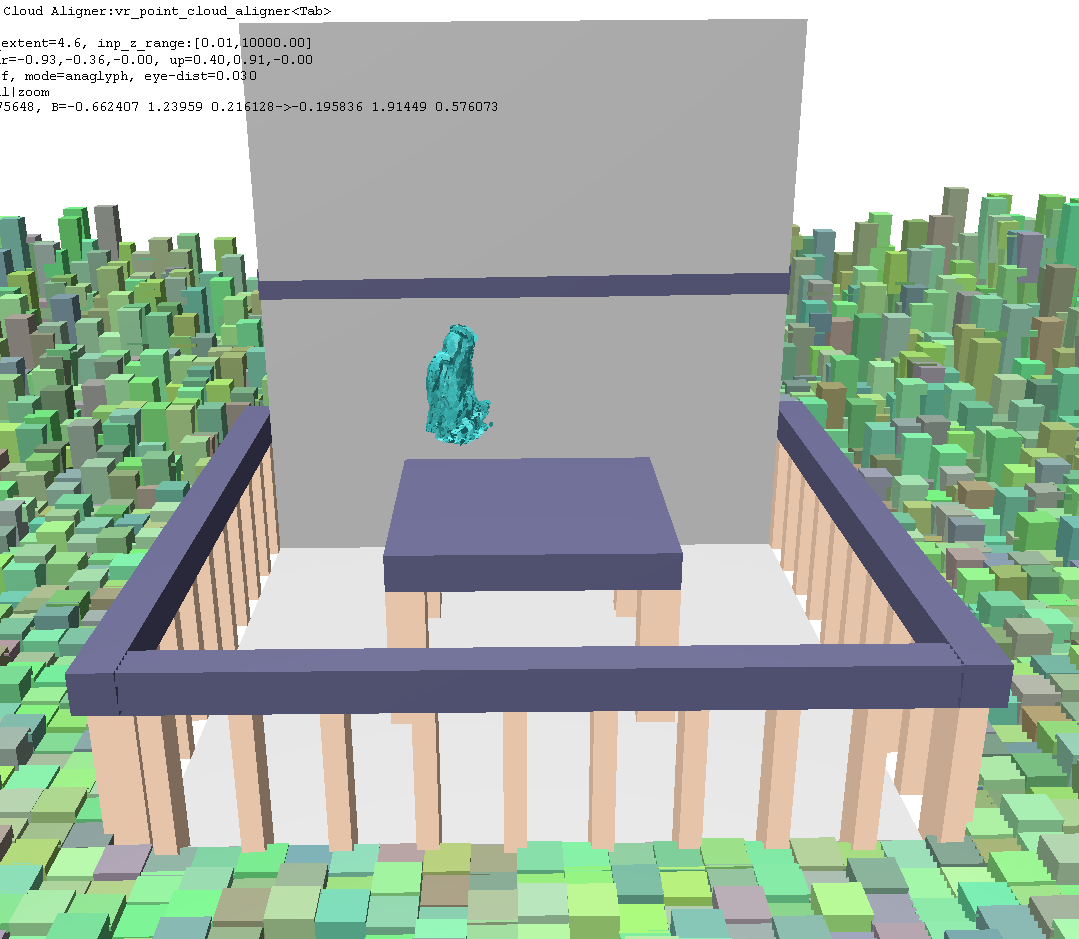
\includegraphics[width= \linewidth]{vrroom.png}
	\caption{The virtual room in its rendered state}
	\label{fig:room}
\end{figure}


 
\subsection{Scaling}

Greater objects may not fit in the room at all and need to be scaled to fit, on the other hand some are so small that the user may have problems to see their important features properly. To give the user the option to adjust his, a scaling function is bound to one of the controllers touchpad and can be used with the drag motion to scale the 3D scan. Additional attention has to be paid due to the fact that scaling the scans will result in scaled translations and rotations. To ensure that the ground truth rotations and translations can be compared with the scaled alignment the inverse transformation hast to be applied to all alignment translations and rotations first. This is easily done by reversing the scaling factor. The scaling function uses a uniform scale matrix as shown below with scaling factor k as well as its inverse on the right side.


\makebox[\textwidth]{
$\begin{pmatrix}
			S_x & 0 & 0 & 0 \\
			0 & S_y & 0 & 0 \\
			0 & 0 & S_z & 0 \\
			0 & 0 & 0 & 1 \\
\end{pmatrix}$	
$\begin{pmatrix}
			1/S_x & 0 & 0 & 0 \\
			0 & 1/S_y & 0 & 0 \\
			0 & 0 & 1/S_z & 0 \\
			0 & 0 & 0 & 1 \\
\end{pmatrix}$
}
\[
S_x = S_y = S_z = k,  k != 0
\]
\section{User centred Design for VR}

When building an VR based application, traditional 2D user interface design cannot be simply adapted to 3D.
Using popups or mouse emulation projected onto the view frustxum of the user constraints interaction to a 2-Dimensional experience which is rather inefficient compared to the possibilities VR could provide.
To include VR Technology to the project, especially the cgv-Framework, new user interaction methods have to be provided and tested. Since the user is the active part of the application, controlling the actions and main methods of the scan alignment process, user centred design (UCD) had to be chosen. 
Human centred design processes for interactive systems, ISO 13407 (1999), states: 
\begin{quote}
"Human-centred design is an approach to interactive system development that focuses specifically on making systems usable."\cite{w3ucdISO}
\end{quote}
There are many aspects of UCD, the following chapters will focus on the definition and examples used in this thesis corresponding application, showing their usage and further features.

\subsection{Constraints and Affordances}

Affordances describe the relationship between an abstract object or goal a user can achieve with the given actions he has\cite{Jerald2015}.
To improve interaction design it is necessary that these affordances are appropriate and the given actions as easy doable\cite{Jerald2015}.
In our application an affordance would be the relation between moving a scan that has been picked by moving the tracked motion controller. 

Constraints on the other hand are limitations of the given actions a user has. This limitations may be necessary to not confuse the user or to simplify the usage of given methods. A user may move a scan by fault out of the trackable area or below the ground. By adding a simple collision detection that prevents the user from moving scans out of these limitations moving scans is less prone to errors. This would be a constraint to the action of moving the scan with the tracked motion controller. In the application moving scans below zero level should not be possible, the scans bounding box is, moved tracked and evaluated. If an action would position any transformed corner point of the box, the translation is stopped and the corresponding controller receives a signal to vibrate. This indicates a violation of physical constraints to the user, preventing him from achieving an unwanted program state with scans hidden below zero ground level. These scans would be invisible and as seen in the tests caused several problems.

\subsection{Visual - physical conflict}

By creating constraints to moving objects out of a given space, a user may experience a so called visual-physical conflict. The hand moving the object may go through an area but the application does not apply the physical appropriate result\cite{Jerald2015}.
To avoid or at least lower the impact of this conflict user-feedback can be used to prevent the user from provoking these conflicts by accident, like a vibrating controller or a warning message. This introduces another section: feedback design.

\subsection{Feedback design}

Feedback is an essential user experience, which should result in information gain about the result or status of a task or object the user interacted with\cite{Jerald2015}.
A use case in our program would be the switching of colours of a scan when its selected or not. A global selection colour (Bright Red) indicates that this object is selected and will be reference point for further actions. Since scan alignment needs at least 2 scans to be practical the application has a 2 step selection:
Selecting the first scan changes its colour to bright red. But when the next scan is selected the first one changes its colour to a less brighter red signalling it is the secondary pick. Applying the alignment now starts an ICP which moves the second picked scan (the one that is now active) toward the first one.

\subsection{Picking}

Working in VR allows the user to reposition scan components as he wishes to every spot. To align them they need to get close together but if they start already close together they do not look ordered and users tend to split them first, to see the individual scans at least before putting them back together. To solve this problem, all scan components start in a line at a fixed height of about 2 meters at one side of the virtual room. Therefore the user can examine the scans separate.
To pick a scan naturally the user could just walk to the side of the room and pick them up there. This would force one to repeatedly walk across the virtual room to the one wall and back to the table in order to assemble the scan by picking the components. To increase the efficiency and to decrease the effort to reach the scans, the tool has a build in drag function and a corresponding ranged pick function. This function works as a so called "extender grab"\cite{Jerald2015} %[JJ indirekt, Mine at al]
and allows the user via box ray intersection to grab a scan which is out of his personal space.
The hand remote "shoots" a ray from its front direction which now is tested in a Bounding box ray intersection function. If it intersects a component this component is picked.

In order for this algorithm to work the box ray intersection with axis aligned bounding boxes has to be defined first.
An axis aligned bounding box (AABB) is a box defined by two points, min and max. These points span a box along all three coordinate axes of the world coordinate system. This box is defined as the minimum sized box which contains all points of the encaspulated object. This technique is often used in raytracing applications to easily determine if a given ray has even the chance to be blocked by the object, saving computational costs of just estimating every possible intersection with every object of the scene. With these boxes it is first checked if the ray could touch the object anyway and the computational expensive intersection method is called only if this first intersection exist.

In our case these boxes can be rotated and translated due to the fact that the user can interact with scans and can translate and rotate them freely. In order to estimate the intersection the ray has first to be transformed to the boxes local coordinate system by subtracting the translation vector from the rays start point and end point and then using the inverse rotation on the results.
After this the ray is now in the local coordinate system and the local intersection is calculated.

This works by defining the bounding box as axis parallel plane stripes, reducing the intersection problem to one dimension. The intersection between this plane and the ray with his origin and direction vector can be expressed as a linear function:
\[
 f(x) = a^* * t + n
\]

t is the velocity of the ray equal to its change over time. This equals to the x,y or z coordinate of the ray direction obtained from the front direction of the controller pose

a is the axis parallel plane stripe projected to the axis. This causes a to be an interval.

n is the x,y or z coordinate of the ray origin which equals the current controller position

If a* is defined for all axes and the formula 
\[
a^x \cap a^y \cap a^z
\]
yields an interval which minimum is the factor needed for the ray origin to travel to the intersection with the bounding box along the ray direction.
The intersection point P is then defined as:
\[
P_I = minimum(a) * raydirection
\]
If there is more than one component in a row that are intersected the one nearest to the user is chosen by using the shortest calculated distance, which equals the minium of interval a. The interval with the smallest minimum is the component closest to the user.

\subsection{Grouped scans}

During the alignment the user may find the correct rotation and translation to align to scans. To save this but also be able to manipulate the scans rotation and translation without destroying the alignment, the user group scans. These groups now work as one scan with a shared Bounding box and shared translation and rotation and colour. If the user tries to pick the scan they both are selected and if he starts an ICP with the selected group and another group, both scans points are used.
This may come unhandy when the scans are grouped incorrectly and now need to be separated again. To solve this an extra function was implemented. This function splits a group by translating them towards the averaged normal directions of their individual points.

By using the cross product of their averaged normalized normal vector and a dynamic vector which is generated out of the amount of the amount of components the group has.
This is achieved by dividing a circle by the number of scans. The resulting angle is used in a rotation matrix around the z axis. By multiplying the matrix with the (1,0,0) vector x times normalized directions are derived.
The rotation matrix is an axis rotation around the z axis and shown below. Note that the same result could be achieved by using a quaternion which represents the same rotation.

\makebox[\textwidth]{
$\begin{pmatrix}
			\cos{ \alpha } & 0 & \sin{ \alpha } \\
			0 & 1 & 0 \\
			- \sin{ \alpha } & 0 & \cos{ \alpha } \\
\end{pmatrix}$
}

To avoid the possibility that bigger scans can overlap even after the split the minimal distance needed to translate the scans without overlapping is calculated using 2 restrictions:
\begin{enumerate}
\item The maximal Bounding box diagonal is equal to the diameter of a circle around the whole component. To avoid overlapping the point to point distance between the middle points of their bounding boxes has to be at least bigger than the maximal Bounding box Length of the biggest Bounding box.
\item The averaged middle point of the whole group $M_a$ and the translated Bounding Box middle points $M_1$ and $M_2$ form a nearly isosceles triangle.
\end{enumerate}
This can be seen in Figure ~\ref{fig:ico}: 

\begin{figure}[htbp]
	\centering
		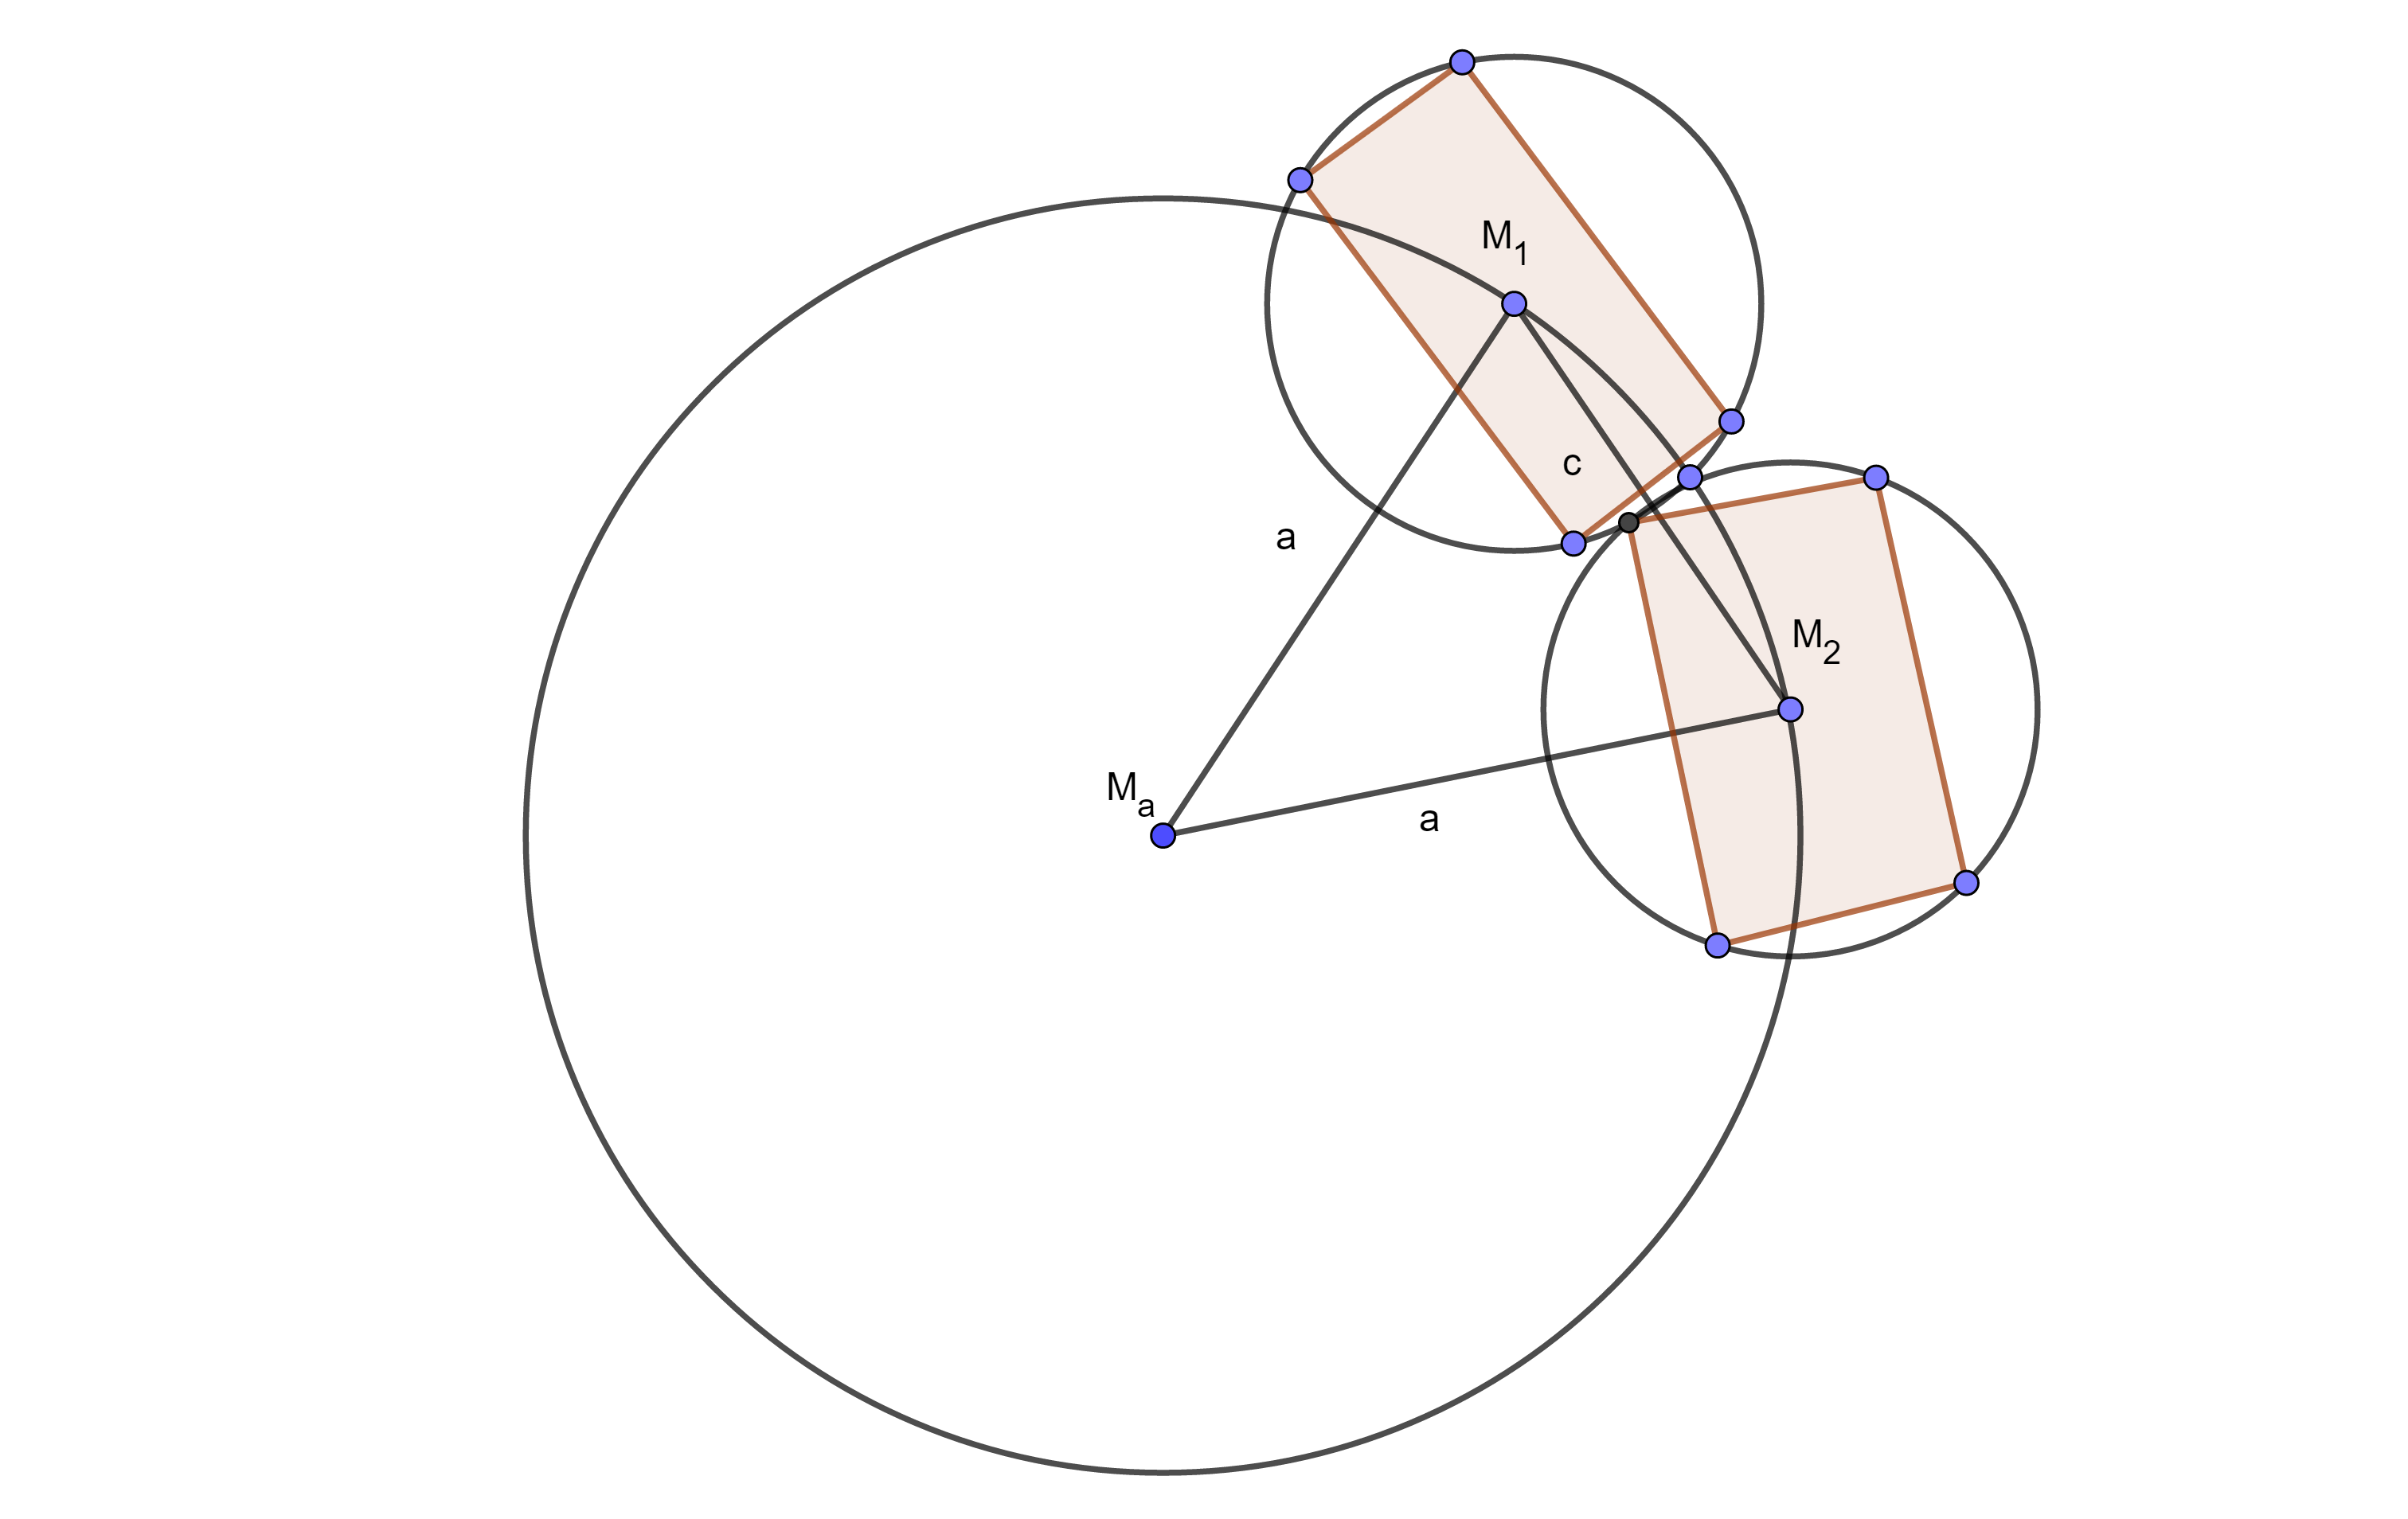
\includegraphics[width= \linewidth]{ico_pic.png}
	\caption{The triangle $M_a$ $M_1$ $M_2$ with c equals the sum of the radius of both circles. Hence the calculation only takes the radius of the bigger bounding box, theside c is well defined as 2r equaling the maximal bounding box diagonal}
	\label{fig:ico}
\end{figure}

Therefore the minimal translation distance from the centre point can be calculated using this formula derived from the formula for icosceles triangles c side by change of constellation.
\[
{\displaystyle  a= {\frac {c}{2 \cdot \sin \left({\frac {\gamma }{2}}\right)}} }
\]
C equals the minimal distance between the middle points of two separate scans, which is equal to the maximal bounding box diagonal. The minimal translation in this formula is represented by a.
The assumption of the program is that the middle point of the scans is near to the averaged middle point of all its points. This is only the case is the distribution of points is evenly among the scans bounding box, and if the bounding box is not heavily deformed due to outliers.
As further suggestion an outlier detection on loading the scans to the program should ensure this restraint.
The application uses a factor of 1.1 of this minimal distance to avoid errors due to the fact that the computer works with floats and doubles which are not always precise and that there may be a distance between the averaged middle point of the group and the middle point of the Bounding Boxes of the scans.
After this splitting translation was executed, the user now can chose a single component out of the group and separate it. The remaining group turns back to its initial state, the separated scan is lifted above the group.

\subsection{Scan positioning}

The most important task of the developed application is to provide a useful toolset, which enables the user to align scan components together. The following functions are responsible for actions that move scans in the virtual environment.

\subsubsection{The reset function}

This function works as a simple reset. The user forces the components to all disasemble and reposition onto the default wall even if their loading position was somewhere other than default. This function is a hard reset even deleting colour and group information.

\subsubsection{The position above table function}

This function is a repositioning function to reposition a picked group to the middle table in the lowest height available. This height is determined by the lowest corner z-coordinate of the lowest bounding box of the group. Additionally the groups averaged middle point is now in the middle of the table, which is by default the middle of the room.

\subsubsection{The loading functions}

These special functions are not directly called by the user. They are instead called whenever the user decides to change the workspace by loading a new project or directory loading. A newly created component always causes the program to initialize its transformations unless they have a flag set that prevents the program from overwriting the transformations. These flags are used in project files to signalize that this is a component the user has already worked with and this should not be repositioned by loading. 

\subsubsection{The reposition execution animation}

To avoid instant teleportation, every repositioning that is not handled by directly grabbing a component thus attaching it to the hand controller, is instead animated as a linear blend between the original translation position and the target translation position. Additionally a second animation executes the rotation (if there is one) at the same time.
These linear blend is executed on colours as well, making hard colour switches only available for blinking animations or the picking event. This is especially important to signalize that blinking colours are indicating that the user has to confirm an action. Additionally the user can see what he caused with his actions instead of a rapid state change of the program. When several translations are executed by one action it could be irritating with no fluent transition to the new state.

\subsubsection{The dragging function}

One of the core functionalities for this application is the possibility for the user to directly "grab" a scan and align it by hand next to the target. In order to work this feature needs several helping functions. The picking method determines the selected scan. If the user holds the picking button, the selected scan is now bound to his controller by the controllers virtual pose. This pose is described as a matrix containing the origin point of the controller in world coordinates, as well as all 3 axes of the controllers coordinate system in world coordinates. By calculating the position of the picked group or component in the local coordinate system of the controller and storing this value dragging becomes possible. The local position is obtained by multiplying the local pose of the component (if it is a group all calculations need to be made per component separately) to the inverted pose of the controller. As soon as the pose of the controller changes, the actual pose matrix is multiplied to the already stored local positions, resulting in a transformation so that the pose of the group or scan in the controllers coordinate system remains equal. The actual result in world coordinates is a transformation as if the scan/group is bound to the controllers picking ray. Additionally the user can change the group/scans local pose towards the controllers z axis. This results in the scan/group coming nearer towards the controller, or further away. This action is triggerd by a scrolling movement on the touchpad. 

\subsection{Controls Mapping}

When it comes to user interaction the VR-Hardware used for this program provides different physical interfaces to interact with. 
The first Mapping was to define a main controller, which has been the right one, due to the fact most people are right handed. Only the main controller is capable of dragging scans and reposition them.
Dragging two groups of scans at the same time could have a negative impact on the framerate of the program, as well as it would obtain one more button from the left controller for a function that is already implemented on the right controller.

The shortage of buttons on the controllers forced the mapping to use both controllers separately for different functions. The trigger of the main controller is the picking button and when pressed and held above the 0.4 threshold acts as dragging controller. As described above the touchpad is limited to only track up and down in order to get groups towards the controller or away. The second touchpad on the other hand is not used, as there is no second function that could use a scrolling functionality. Additionally this scrolling motion would get triggered every time the press function is used on this touchpad. To not mix up scrolling and pressing function on touchpads, the right touchpads pressing buttons are not used, instead the left ones are used. The first function is to position the picked group above the table (UP), which should enhance the intuitiveness by connecting the up button with a function that positions scans mostly upwards. Additionally the restore the last state or abort (left) and restore back (right) are on the same touchpad and ordered in opposite directions to sharpen the contrast of their inverse functionality. The downward button was once mapped to start the ICP but this was removed.

The menu button of the main controller is bound to the uniting action. This merges two groups to one group as the right controller is designed to drag scans and interact more with the scans, the merging action should be mapped to the same controller.
The menu button on the other controller however, is mapped to the exact opposite of this action, it opens the separation selection. As the menu button is the one button thats most difficult to reach after the hard to press grip button, accidentally disasembling a aligned group should not happen.
The reset function is mapped to the left grip button. As this function should not be called and is only there for debugging purposes or if the user really does want to erase his progress, this function got mapped to the button that is hardest to press and not called by accident.
In order to avoid confusion or accidental use of the reset function, the right grip button is not used. This way users may not confuse the button with its pendant on the right side containing the reset function. For safety the restore latest state function can undo the reset function.

\subsection{Additional application concepts}

Some features of computer programs have evolved over the time and it is common to include them to all applications because of their general purpose. For example the possibility to restore the program state before the last action is a well known feature and commonly expected to be in every program. %(FIND QUOTE)
This feature is implemented by a vector which tracks all program states since the last project loading was called. If the user now decides to reverse his last action, the vectors latest pushed state is loaded and restored. Additionally the possibility to reverse this is included as well. The vector then only restores the i+1 th state after the actual program state if this state exists. By reversing a state, then pushing a new state via a specific action the old i+th state will be deleted to avoid state inconsistency.
The repositioning of scans due to reversing or restoring actions triggers an animation as well. This animation is similar to the one used in the reposition execution animation and applies to colours, rotations and translations.

\chapter{Interactive VR-user study}

To examine the capability of coarse alignment systems in VR a user study has been conducted. In order to work properly the programs starting state for this study has been designed beforehand. The first part of the study included a short introduction to the handling the VR environment as well as a short phase for all test persons to explore and test the features the program delivers. In the second part the the test persons are encouraged to align a ground truth dataset provided by the chair of computer graphics as exact as possible by hand. %Chair?
There is no time limit for this process the user decides wether he is finished or not after all scans are in one group. During the execution of the test, feedback for questions with the handling is allowed, due to the fact that a user may not memorize all functions of the program after the introduction.

Afterwards every test person is asked to fill out a short form to evaluate the usability of the program for further improvements. The used form can be found in the Appendix, see ~\nameref{sec:appendixform}.

\section{Test setup}

The tests took place in the Holodeck room of the faculty of computing since. In this room the tracking stations were set up in two corners of the room diagonal to each other. The trackable area was sized to fit at least 3.5 x 3.5 meters and has a real table in it to emulate the virtual table. The exact measurement of the table was estimated beforehand and the program was initialized with the exact virtual copy of this table. The users now interact with a virtual projection of a real existing table.

The full test setup from above can be seen in figure ~\ref{fig:test}

\begin{figure}[htbp]
	\centering
		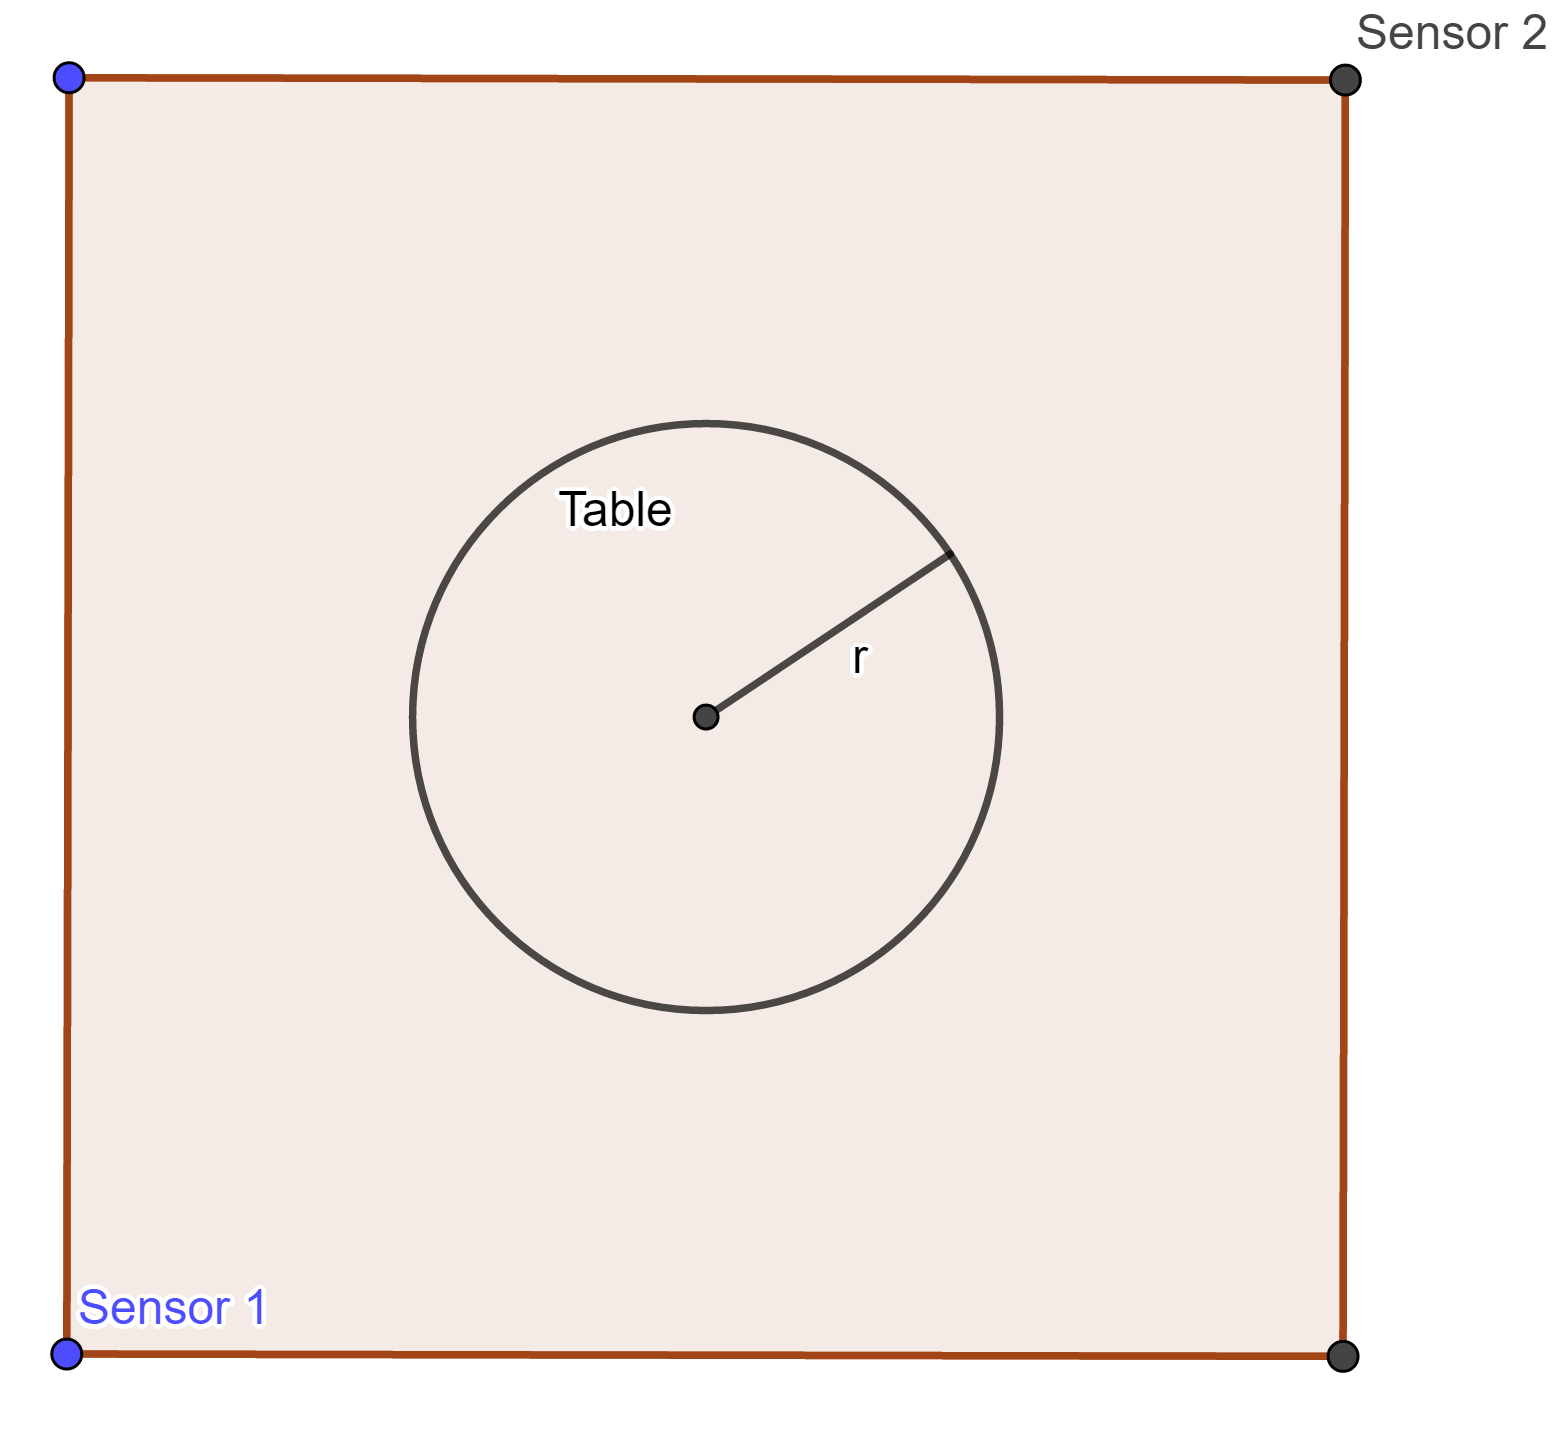
\includegraphics[width= \linewidth]{test_setup.png}
	\caption{The test setup from a top down perspective}
	\label{fig:test}
\end{figure}

In the virtual environment all tests scans are located on a height of about 1.8 meters floating at the left wall. The user now can drag them onto the table or use the selection and positioning function to directly put a selected scan onto the middle of the table.
The dataset used for this test the owl data set which contains normals and a known ground truth alignment. Scaling had to be set to x, so that the seize of the owl is about 0.7 meters high.

\subsection{Equipment}

The complete setup uses two vive hand controllers, each with a touchpad, an analogue trigger, a menu button, a grip button and the touchpads themselves have four press-states (up,right, down left). The system button can not be called by the program, it will always bring up the steam menu and is therefore not included as interaction. The two tracking stations are mounted at eh ceiling of the room in about 6.25meters distance, which is a bit too much for the optimal distance that is suggested by valve. The head mounted display (HMD) is attached to a computer on the north side and has about x meters cable length, enough to reach every corner of the room. To avoid possible problems with the cable twisting around the user, the supervisor always keeps track of the cables situation during the experiment.
The used pc for this study was a four core machine (Intel i5 2700k) with a Nvidia GeForce 1060 GTX graphics card. The capability of the system to provide a 90Hz picture with a constant framerate and no framedrops was tested before and was monitored during the tests.

\subsection{Guidance}

Before starting the tests users were introduced to the program in a short explanation and summary what they will do and what is expected. There was no time limit set in order to let the user take their time for more precise alignments. During the tests constant feedback for questions was guarantueed by the test supervisor and the mappings of features could constantly been asked for.

\subsection{Tracked metrics}

The program constantly records user interactions in the programs state vector, but due to the fact that by reversing actions some reversed actions may be deleted and not recorded any more an additional change stack was introduced. Every user interaction that caused a program state change is pushed back to the stack and counted as well as differentiated by the kind of state change. These state changes include: scan pick, scan drag, scan unite, scan separate, repositioning above table, reverse action, restore action and the hopefully not to be used reset function.
Additionally the time the test person needed to align the scans is measured too.
The most important metric however is the accuracy which is calculated afterwards. The project allows to save all translations and rotations to a special file format called transformations project file (.tpj). This contains the file path for unambiguous identification of the component along with the translation vector and the rotation in quaternion representation. The ground truth data is then scaled identically to the scaling used by the test, otherwise the results would not be usable as both transformations would be saved with different scalings.
Then the two error metrics average translation error and average rotation error are calculated by a function when saving the user generated tpj file and written there as output. The calculation steps are explained in the next section.

The last metric usability is a subjective metric which was obtained by a short form users filled out after the test. 

\subsection{Calculation of translation and rotation Error}

When calculating these metrics, several problems have to be considered. The translation and rotation information accessible from the program are in world coordinates. Simply calculating the difference between the aligned data and the test data would result in a not reliable metric, as this would depend on the orientation and position of the aligned data in the virtual world. A simple approach to handle this problem is to selecting one component of the ground truth data and calculate the transformation of this to the corresponding component of the aligned data. This is a more reliable metric but still would result in having a direct dependency between the accuracy of the selected component and the rest of the components towards only this component. The general accuracy between all components to another would not be considered. 
In order to objectively calculate an error metric that does not rely heavily on one specific component, the following method was considered to be the best. The program calculates the relative pose of 2 components of the ground truth data and the corresponding components of the aligned data. Then both results which are relative poses are compared. 
To do this the rotations of both components, represented by their quaternions $q_1$ and $q_2$ are used to calculate a third quaternion $q_p$ which represents a rotation from one component to the other. This is done by using the formula with the inverse of the first rotation and the second via field multiplication:
\[
q_p = q_1^{-1} * q_2
\]
This way the relative poses of the two components rotationwise are derived for both ground truth data $q_{p'}$ and test data $q_{p'}$. Then the difference between both poses, ground truth and test data can then be calculated with the same formula resulting in the quaternion $q_e$ which represents the rotation needed to rotate from ground truth to test data. As a quaternion itself is not a good metric to compare, the error quaternion $q_e$ is transformed to axis rotation representation. The angle of the axis rotation is then the error metric. 
The following formula extracts this angle out of the quaternion by using the real part re of $q_e$:%REALPART?
\[
	\alpha_e = 2 *  acos ( re )
\]

The translation vectors are more difficult to retrieve, as they depend on the corresponding orientation of the component. In order to resolve this dependency the differential vectors need to be orientated to world coordinates. To get a vector between the two poses of the components, the first translation (origin) needs to be subtracted from the second translation (destination). The destination determines the direction of the vector in the room therefore needs to be oriented to world coordinates. To ensure the translation differences of ground truth and test data are in the same coordinate system, the resulting difference vector has to be rotated inverse by their corresponding rotation of the destination component. Figure 4.1 shows a sketch of the described procedure.

After retrieving the rotation and translation error from one component to another, the same procedure is repeated for each component, resulting in a vector of $N^2$ values. N is the number of components the dataset has. Out of these values the mean is calculated and taken as the final result, shown in the formula below
\[
\frac{\sum_{i=1}^{N}error}{N}
\]

\section{Test results}

The the results of the error metric calculation are shown in the following table, in line with other useful information:

\begin{table}[!h]
\begin{tabular}{|l|l|l|l|l|} \hline
Nr & mean translation error (mm) & mean rotation error (rad) & needed time (min) & total user actions \\ \hline
1 & 102.7 & 0.161078 & 6:49 & 409 \\
2 & 90.1727 & 0.135561 & 9:26 & 275 \\
3 & 123.615 & 0.169968 & 12:34 & 460 \\
4 &  &  & 21:22 & 611 \\
5 & 77.8557 & 0.114094 & 7:12 & 210 \\ \hline
\end{tabular}
\end{table}

Due to a bug during the execution of application Nr 2, 3 and 4 have had an extra calculation which did not consider one or two components. See chapter Problems for more details.
The total of user actions consists of every user interaction with the vive system, whether it was successful or not. This does not include the interaction of changing the position of the HMD or controllers, but does include every key that was pressed and is used in a function.
Participant number five is the application author and will thereby only be considered as reference to optimum usage.

\chapter{Evaluation}

This chapter will interpret the test results as a first step. Then a short analysis of these results is done for both, the registration aspect as well as the user interaction aspect. At the last part of this chapter, an evaluation of these results will lead to the decision wether this experiment was successful or not.

\section{Analysis of error metrics}

The results show a clear convergence to more correct results when the user has already had experience with a VR system at all. Test person one, two and five were most experienced with VR systems and had worked with them before. Test person 3 and 4 were completely new to such systems and therefore least accurate. The accuracy of results is actually close the semi automated method by Chao \cite{Chao}, as their average error was around 50mm before applying an ICP. The tested results show a translation error in between 70 to 120 mm achieved in less than 15 minutes in average. The total time used by Chaos method was estimated to be around an hour\cite{Chao}. Although these results are not comparable, because of the usage of different amounts of points and scans, these numbers show that the tested method can achieve a good coarse alignment in a tenable time.

By taking a look at the rotation error, the results show an astonishing tendency to be quite accurate for a manual alignment, as their average is in between 0.11 to 0.16 rad equally to 6\textdegree to 10\textdegree. This should be more than accurate enough to apply a fine registration algorithm afterwards, such as the ICP. The rotations generally show more accuracy than the translations, the reason is that a small translation error between 0 and 10 centimetres does not significantly disturb the composed point cloud in its appearance, whereas rotations that are incorrect show a greater impact on the appearance. An observation that was made is that if scans are aligned from the view of one side, an error was less easy to detect. Test person Nr 4 assembled the point cloud about one meter apart from their view point. The result was that from that perspective the alignment seemed good, but when taking a look 90\textdegree from the side the alignment was not well. Upon examining the exact calculated results componentwise there was a trend that components from the top side where near together, components from the back side as well, but both group had a significant distance between them. This distance could only be seen from another view point. This shows that the perspective problem is also present in VR, the expense to change the Viewpoint in VR is to walk at least about the length of the point cloud.

\section{Analysis of user interactions}

The user interaction Analysis is splitted into two parts, first an examination of the raw data of the user interaction tracker system used for the experiments, the users feedback is included in the second part.

The tracker system implemented counted every different action, the type of actions and their usage by the test persons are shown in the table below.

\begin{table}[!h]
\begin{tabular}{|l|l|l|l|l|l|} \hline
Action type & 1 & 2 & 3 & 4 & 5 \\ \hline
Component dragging & 157 & 103 & 160 & 210 & 97\\
Component picking & 216 & 103 & 239 & 210 & 97\\
Component deselect & 8 & 48 & 30 & 178 & 0\\
Group separation display & 7 & 0 & 2 & 0 & 0\\
Group separation confirm & 3 & 0 & 1 & 0 & 0\\
Reverse last action & 2 & 8 & 8 & 0 & 2\\
Restore last action & 0 & 0 & 0 & 0 & 0\\
Position above table & 0 & 0 & 0 & 0 & 0\\
Reset & 0 & 0 & 4 & 0 & 0\\
Unite groups & 14 & 13 & 16 & 13 & 14\\
Total of changed states & 262 & 169 & 243 & 308 & 157\\ 
Total actions & 409 & 275 & 460 & 611 & 210\\
\hline
\end{tabular}
\end{table}
The total of actions needed for an alignment were never lower than a total of 200 actions. The count of total actions differs more or less widely to the total of changed program states, indicating an difference between actual valid actions that cause a program state change (e.g. picking a new component, repositioning it, or using any other of the functions in a valid way). The optimum for this metric would be a one to one relation, which indicates that the user never made mistakes and the workflow was as optimal as it gets. The high count of picking and dragging actions is the result of a missing rotation functions, leading to the problem that the dragging function had to be called several times in order to rotate a component. In the feedback paper two of the participants noted that an extra rotation functionality to rotate a picked scan around the normal axis of the picking ray would improve the usability. More obvious was that the function that repositions the picked group on the table was never used. All users identified this functionality as least useful after the experiment. The group separation was also not often used but still considered to be usefull.

The deselection functionality was mapped to the same button as the picking function but on the other controller, leading to confusion of some of the users, as they expected to pick scans with both hands. If the user is already trained in handling the application, the deselection function becomes even obsolete, proven by the optimum usage of participant number 5. 

Surprisingly the difference between changed states, and total actions was not lowest for the reference participant five, but for test person two, as the difference is only 13. The  high difference for the other test persons leads back to the functionality of deselection and picking: When used several times on the same target in short time intervals the action does not count as valid, as it does not change anything. The reason this happens often is because the picking and deselection is mapped to the trigger of the controller, its values can fluctuate around the threshold causing the program to register up to 60 trigger events per second. From this events on average 10 are exceeding the threshold in one way and cause the application to register all of these as actions. Because they do not change the program state, they are not counted as valid. To avoid this problem in future experiments, a timer event that blocks the picker for some milliseconds after the first valid action could be implemented. This avoids that the fluctuation zone around the trigger threshold causes the controller to constantly activate the event counter.

The general feedback after the experiment was positive, most functionalities were rated useful by the user. Especially the reverse action though not often used was particularly mentioned in this context. However the critique was mostly about bugs that were still in the program during the experiments. The picking function falsely worked in both directions, so if the user picks a scan in front of him, while the controllers back direction was pointing towards a scan behind it, the application selected the scan behind the user. This lead to a lot of confusion and extra work, in some cases users accidentaly pushed these scans out of sight or through the walls of the virtual room. Due to lack of time the functionality that blocks scans from being pushed outside the virtual room was not finished. In two experiments this lead to a scan being completely out of sight and these had to be ignored during the calculation of the error metrics, lowering their reliablity. As mentioned before the second point was the missing rotation function.

Other points which had been concerning, like the hand to controller mapping accuracy, where mostly not a problem for users. Users perceived the mapping and tracking of the controllers as natural and rated the accuracy good. The separation selection used by test person number one was criticised for not changing the colours before the animation starts, so that the user can identify the wrong aligned scan before they traverse apart. The animation duration was considered to be too long and should be shortened.

\section{Experiment conclusion}

The accuracy of alignment and time needed for this show that the concept of coarse alignment via VR has potential. Furthermore its full potential once a fine registration alignment method is included, which drastically shorts the amount of time a user needs to reposition scans   should be considered to be even higher. Even users with little experience could align components accurate enough to execute a fine alignment algorithm afterwards. If a surface reconstruction is added users may even be more accurate due to the fact that the point clouds were only visible due to the fact that their points were shown with a width of 5 pixels. Further experimentation with an improved version of the application could show even better results.

As for the user interaction the general concepts were perceived good by the users. Concluding the users feedback a general improvement would be a rotation function during the dragging of a scan is active. A possible realisation would be to map this function on the touchpad of the dragging controller, but the user can swipe right or left or right to rotate the object around its y axis. Additionally all scans should be oriented, so that the actual top side of the scan shows towards positive y direction. This way rotating is only needed around the y axis. In order to balance conflicts with the dragging towards (or away) functionality, an intelligent tracking system of the touchpads changes should prioritize the dominant swiping movement instead of performing both, translation along the controller ray and rotation around the components y axis at the same time.

The suggestion to enhance the separation process by colouring the components before translating apart is considered to be very useful and should be included too.

As last point for improvmement a general fix of all still occuring bugs should be prioritized as they have the greatest impact on the user interaction.
The experiments have shown that the application and the user interaction concept were successfull, but have minor issues that could be adressed easily.

\chapter{Problems}

This chapter adresses problems that occured during all stages of this thesis and their impact on the final application that was developed.

\section{Implementation problems} \label{ch:Problems}

In order to enhance the real time compability as well as the general accuracy of the used ICP methods, a public open source code library of the stanford university was used and integrated as header file. Unfortunately this library had a lot of issues with the underlying dependencies and was not perfectly compatible to the framework. As for the sparse ICP implementation results were nowhere near usable, the alignments were diverging instead of getting closer. The basic point to point method which used iterative reweighting
was more accurate. Unfortunately this method often failed to align scans due to finding local minima which were incorrect. The missing numerical stability included the possibility to produce INFINITE vectors or even NAN results.

The real time requirement restrained the usage of more complex variants with refined error metrics due to the fact that the running time would increase significantly. Final tests in the actual application with the vive showed that the calculation time increased as well due to the complexity of handling a complete framework which renders a 90Hz stereoscopic view for the Vive and has to handle at the same time polled events of the technical devices such as pose events, button events and further more. As the usage of the ICP with more complex scans than the initial test set (the drill scan from the stanford 3D scan repo) completely failed to work in real time with subsampling and even failed to proper align without subsampling, the ICP has been cut out of the program.

\section{Hardware problems}

The maximum recommended distance between the two tracking stations of the vive system turned out to be below the actual distance. This may caused some problems such as tracking to be less accurate. The result of that is more difficult control of the scans when dragging. As the main aligning operation is dragging and turning the scan with the controller, less accuracy of tracking can lead to less accuracy in alignment. This may distort the accuracy metrics used in this paper. Due to the fact that these trackers need to be mounted to the ceiling to work, changing their position in the room is not possible in this case. As the distance was only a recommendation and tracking seemed very accurate at any time of the tests the problem has been discarded from consideration.

\section{Time shortage}

The bug situations with the ICP function caused a great time delay during the end phase and the late finishing of the VR binding added an additional delay to the time planning. In the end this lead to a time shortage that forced the cut of the ICP feature as well as a shorter debugging time with the VR system before the experimental setup. This resulted in a not bug free but still working test environment with much room for improvement. Concluding from these events an improved strategy would be to move earlier from the 2D envornment used for testing and adding features to the full VR environment. Some concepts that worked well in the testing area, like the positioning above the table, as dragging and moving was very difficult there, were completly useless in VR. The experiments should have been tested earlier with VR in order to rethink some of the added features, or to find missing features. Additionally a self implemented version of an ICP based on the widely used Eigen libraries would have worked better than the versions that were found online and incompatible with the framework. This way the subsampling function could be integrated directly into the ICP and further improved the requirements of real-time and accuracy. On the other hand this would cause another delay and even exceed the demandable work for a bachelor thesis.

%[https://www.vive.com/us/support/vive/category_howto/what-is-the-recommended-space-for-play-area.html]
%

\chapter{Conclusion}

For this chapter the thesis problems are reviewed and checked if they were resolved and if not what additional steps are necessary. 
The literature reasearch on interactive registration methods was done in the first chapter about 3D registration, but is very short due to the fact that there are not as many interactive approaches to the problem of 3D scan registration. However it was enough to gather information from comparable work and use this information to avoid similiar problems during the experiments.

The collection of a representative set of 3D scans was provided by the char of computer graphics of the TU dresden. During the first test phases the 3D scan repository of the university of stanford was used. Mainly the well known stanford bunny but as well the drill scan, which has very few points and was especially usefull during debug mode.

The Design of a VR environment was successful and as the experiments have shown an interactive registration was not only possible but also efficient. The average time needed for a full alignment was a bit above ten minutes and users of the application rated it as efficent and positive with some minor missing details.The picking and positioning strategy was successful and turned out to be intuitive and easy to pick up for most users. A small improvement on the way rotation can be adjusted was missing.

The strategy and development to guide the users was cut short due to a lack of time. Instead an oral introduction to the process has been given before each experiment, which was enough for all users to fullfill their task. However test persons mentioned that they were missing a way to see the controlls and had to ask sometimes if they forgot a function. As a concept an reconstruction of the controller with small icons on every button should be considered. These icons should give a hint what functionality the specific button has and would help the user to understand the features. Additionally a short introduction clip or popup should instruct the user to what his or her task is. With these additions a supervisor explaining everything at the beginning would become obsolete.

The automatic fine registration algorithm could not be included as statet in the chapter implementation problems. A possible solution is an own simple version of the ICP that uses the already implemented subsampling methods and could work more efficent than third party provided software. Because the coarse alignment generated from user input is quite accurate the ICP would not need to be as strongly optimized as other versions that are used in fully automated registration software. This would also enable real time calculations of the fine registration, as in this interactive system a long ICP calculation would lock down user interaction during that time.

The evaluation and conducting of a qualitative user study was performed with success and proved that the concept of an interactive 3D scan registration software can work. The application developed during this thesis needs some small improvements and additions and then could be tested again with more conditions and an higher accuracy.

Due to the time shortage no optional tasks were fulfilled.

The concepts used in this thesis can be applied to several fields of usage. As already mentioned in related work some fields of application like medical scans already need a person as supervisor to check the scans produced by machines. In this field an efficent interactive registration method for MRT and other medical scans may be useful replenishment to enhance the processing of these scans. In order to refine this method further research in improvements to the application is needed.
As a second possible field of use the gaming industry may use these developed methods and concepts for 3D virtual puzzle games, as there is now the possibilty to create more complex and challenging puzzle of real 3D scans that the user now can align. As mentioned by all participants of the study, the general experience was interessting and some also mentioned that they did enjoy the task to put together a 3D scan, though even it was nothing more than a point cloud in that time. By adding a more realistic environment and even surface reconstraction as well as textures the application could provide a game like experience.

My own impression of the application is that with addition of several features and improvments i assume that an additional study could provide interesting insights to the concept of interactive 3D scan registration.

\chapter{Appendix}

\section{Diagramms and statistics}

\begin{figure}[htbp]
	\centering
		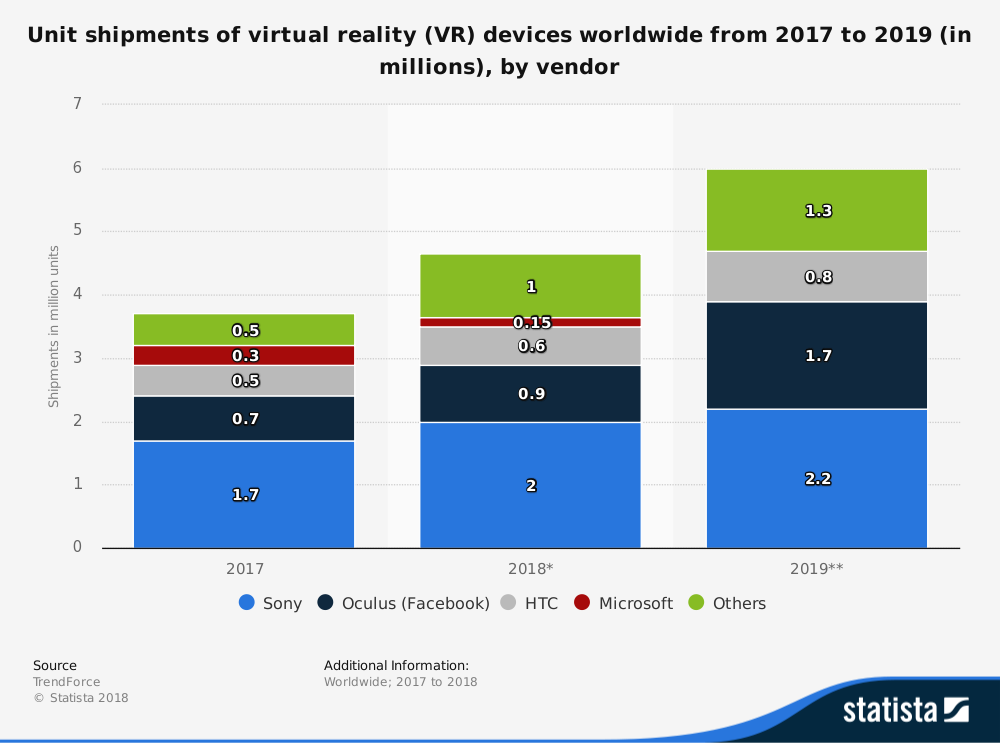
\includegraphics[width= \linewidth]{sales.png}
	\caption{Shipments of VR devices worldwide from 2017 to 2019, *Estimate **Forecast, Source: Trendforce}
	\label{fig:sales}
\end{figure}
\newpage
\section{Survey form}
\label{sec:appendixform}
{\centering \textbf{Interactive VR study survey}}

\textit{Please answer the questions with a tick on the right side, by selecting one box. 5 stands for the lowest grade while 1 is the best grade.}

\begin{table}[!h]
\begin{tabular*}{\linewidth}{l@{\extracolsep{\fill}}|l|l|l|l|l|} 
\parbox[t]{10cm}{} & 5 & 4 & 3 & 2 & 1 \\ \hline
\parbox[t]{10cm}{How was your your general experience with the VR application?} & & & & & \\ \hline
\parbox[t]{10cm}{How would you rate the virtual environment designed for this application?} & & & & & \\ \hline
\parbox[t]{10cm}{During your time in VR, how natural felt the mapping of your hands into the VR space with the controllers?} & & & & & \\ \hline
\parbox[t]{10cm}{How well did the introduction and guidance at the beginning prepared you for your task?} & & & & & \\ \hline
\parbox[t]{10cm}{How accurate would you estimate the tracking of the Vive system during your time with the application?} & & & & & \\ \hline
\end{tabular*}
\end{table}
\textit{These questions can be answered by text or short notes.}

Did you miss any feature/functionality of the application during the alignment of the scans that could have helped you with your work? If yes please describe shortly which.

\noindent\makebox[\linewidth]{\rule{\linewidth}{0.4pt}}

Was the set of functions prepared to help with the alignment useful? If yes did you use all of them?

\noindent\makebox[\linewidth]{\rule{\linewidth}{0.4pt}}

Which of these functions did you need the least?

\begin{tabular}{l r}
-> The one that positions the picked group above the table and centers it & O \\
-> The one that reverses the last action & O \\
-> The one that separates a scan from an assembled group & O \\
\end{tabular}


Which parts/functions of the application you were unsatisfied with and should be improved? 
(Leave empty if there is none)

\noindent\makebox[\linewidth]{\rule{\linewidth}{0.4pt}}
\noindent\makebox[\linewidth]{\rule{\linewidth}{0.4pt}}
\noindent\makebox[\linewidth]{\rule{\linewidth}{0.4pt}}

Thank you for your time!


\end{document}